% !TEX TS-program = pdflatex
% !TEX encoding = UTF-8 Unicode
% {{{ setup
\documentclass[a4paper]{article}

\newcommand*{\ShowReferences}{} % Comment to hide the References.
%\newcommand*{\ShowGlossary}{} % Comment to hide the Glossary.

\newcommand{\doctitle}{{Boring Flops: Some Opinions on Synthesisable RTL}}

\usepackage[pdftex,pdfauthor={Dave McEwan},pdftitle={\doctitle},breaklinks,hidelinks]{hyperref}


\usepackage[a4paper,margin=2.5cm,headheight=13.6pt]{geometry}

% setup_misc.tex
% Just provide some convenient environments.
% Nothing in here should make sweeping changes to layout or the overall look.

% Place a horizontal rule.
\newcommand{\Hrule}{\hfil \rule{0.67\linewidth}{0.4pt} \hfil \\}

% Temporary note highlighting TODO.
\newcommand{\TODO}[1]{[\textbf{TODO} \textsl{#1}]}

% Just a nice way to typeset the word BibTeX.
\def\BibTeX{{\rm B\kern-.05em{\sc i\kern-.025em b}\kern-.08em
    T\kern-.1667em\lower.7ex\hbox{E}\kern-.125emX}}

\usepackage[utf8]{inputenc}

\usepackage{ifthen}

% Put pages landscape in PDF.
% http://mirror.ox.ac.uk/sites/ctan.org/macros/latex/contrib/oberdiek/pdflscape.pdf
% \begin{landscape} ... \end{landscape}
\usepackage{pdflscape}

\usepackage{grffile} % Allow dots in filenames.

\ifdefined\NoGRAPHICX \else
\usepackage{graphicx}
\graphicspath{{./}{./img/}{./shr/img/}}
\fi

% \fref and Fref for nicer references.
\usepackage[english]{babel}
\usepackage[plain]{fancyref}
\vrefwarning % NOTE: Comment and check errors before releasing documents.
\newcommand*{\fancyrefapplabelprefix}{app}
\fancyrefaddcaptions{english}{%
  \providecommand*{\frefappname}{appendix}%
  \providecommand*{\Frefappname}{Appendix}%
}
\frefformat{plain}{\fancyrefapplabelprefix}{\frefappname\fancyrefdefaultspacing#1}
\Frefformat{plain}{\fancyrefapplabelprefix}{\Frefappname\fancyrefdefaultspacing#1}
\frefformat{vario}{\fancyrefapplabelprefix}{\frefappname\fancyrefdefaultspacing#1#3}
\Frefformat{vario}{\fancyrefapplabelprefix}{\Frefappname\fancyrefdefaultspacing#1#3}

% Text Companion fonts for text symbols.
\usepackage{textcomp}

% Greek letters in text mode without changing to math mode.
\usepackage{textgreek}

% Algorithm typesetting environment.
% \begin{algorithm} ... \end{algorithm}
\usepackage{algorithmic}

\ifdefined\NoXCOLOR \else
% Lots of commands to control color.
% http://mirror.ox.ac.uk/sites/ctan.org/macros/latex/contrib/xcolor/xcolor.pdf
\usepackage[usenames,svgnames]{xcolor}
\fi

\ifdefined\NoENUMITEM \else
% Allow list customization (enumerate, itemize, description).
% http://mirror.ox.ac.uk/sites/ctan.org/macros/latex/contrib/enumitem/enumitem.pdf
\usepackage[shortlabels]{enumitem}
\fi

% Define the \FloatBarrier command.
\usepackage{placeins} % \FloatBarrier

% Extensions to the tabular environment.
% Cells which can span multiple rows.
\usepackage{multirow}
\usepackage{makecell} % \thead and other macros for table cell formatting.
\renewcommand\theadalign{bc}
\renewcommand\theadfont{\bfseries}
\renewcommand\theadgape{\Gape[4pt]}
\renewcommand\cellgape{\Gape[4pt]}
\usepackage{longtable} % Tables split over multiple pages.

\ifdefined\NoTIKZ \else
% Drawing in LaTeX.
\usepackage{tikz}
\usetikzlibrary{shapes, shapes.arrows}
\fi

\ifdefined\NoGLOSSARIES \else
% Typeset abbreviations using glossary.tex.
\usepackage{glossaries}
\makenoidxglossaries

\newglossaryentry{naiive}{
  name=na\"{\i}ve,
  description={
    is a French loanword (adjective, form of naïf) indicating having or showing
    a lack of experience, understanding or sophistication
 }
}

\newglossaryentry{ImageNet}{
  name={ImageNet},
  description={
    is an ongoing research effort to provide researchers around the world an
    easily accessible image database.
  }
}

\newglossaryentry{DutyFactor}{
  name={Duty Factor},
  description={
    Fraction of period where signal is high.
  }
}

\newacronym{ad}{AD}{Adaptive Design}
\newacronym{ai}{AI}{Artificial Intelligence}
\newacronym{amba}{AMBA}{Advanced Microcontroller Bus Architecture}
\newacronym{api}{API}{Application Prognamming Interface}
\newacronym{arm}{ARM}{Acorn RISC Machine Holdings Plc}
\newacronym{ascii}{ASCII}{American Standard Code for Information Interchange}
\newacronym{aws}{AWS}{Amazon Web Services}
\newacronym{AXI}{AXI}{Advanced/ARM eXtensible Interface}
\newacronym{ASIC}{ASIC}{Application Specific Integrated Circuit}
\newacronym{bn}{BN}{Belief Network}
\newacronym{BNN}{BNN}{Binarized Neural Network}
\newcommand{\bp}{BytePipe}
\newacronym{bpf}{BPF}{Band-Pass Filter}
\newacronym{BSC}{BSC}{Binary Symmetric Channel}
\newacronym{cam}{CAM}{Content Addressable Memory}
\newacronym{CDF}{CDF}{Cumulative Density Function}
\newacronym{CMF}{CMF}{Cumulative Mass Function}
\newacronym{cisc}{CISC}{Complex Instruction Set Computer}
\newacronym{CMOS}{CMOS}{Complementary Metal Oxide Semiconductor}
\newacronym{CNN}{CNN}{Convolutional Neural Network}
\newacronym{cpd}{CPD}{Conditional Probability Distribution}
\newacronym{CPU}{CPU}{Central Processing Unit}
\newacronym{CSV}{CSV}{Comma Separated Values}
\newacronym{CTF}{CTF}{Common Trace Format}
\newacronym{DAG}{DAG}{Directed Acyclic Graph}
\newacronym{DDR}{DDR}{Double Data Rate}
\newacronym{DFF}{DFF}{D-Type Flip-Flop}
\newacronym{DFT}{DFT}{Discrete Fourier Transform}
\newacronym{dftst}{DFT}{Design For Testability}
\newacronym{Dkl}{$D_{\text{KL}}$}{Kullback-Leibler Divergence}
\newacronym{dma}{DMA}{Direct Memory Access}
\newacronym{dsm}{\textDelta\textSigma}{Delta-Sigma Modulation}
\newacronym{DSP}{DSP}{Digital Signal Processing}
\newacronym{dtft}{DTFT}{Discrete Time Fourier Transform}
\newacronym{dvfs}{DVFS}{Dynamic Voltage and Frequency Scaling}
\newacronym{ea}{EA}{Evolutionary Algorithm}
\newacronym{eeg}{EEG}{electroencephalograph}
\newacronym{evc}{EVC}{EVent Configuration}
\newacronym{FEC}{FEC}{Forward Error Correction}
\newacronym{FFNN}{FFNN}{Feed-Forward Neural Network}
\newacronym{FFT}{FFT}{Fast Fourier Transform}
\newacronym{flit}{flit}{Flow Control Digit}
\newacronym{fifo}{FIFO}{First In First Out}
\newacronym{fmax}{$f_{\text{max}}$}{maximum operating clock frequency}
\newacronym{FSM}{FSM}{Finite State Machine}
\newacronym{ops}{Op/s}{Operations Per Second}
\newacronym{fir}{FIR}{Finite Impulse Response}
\newacronym{FOSS}{FOSS}{Free Open Source Software}
\newacronym{FPGA}{FPGA}{Field Programmable Gate Array}
\newacronym{ga}{GA}{Genetic Algorithm}
\newacronym{GPIO}{GPIO}{General Purpose Input Output}
\newacronym{HCI}{HCI}{Human-Computer Interaction}
\newacronym{hdl}{HDL}{Hardware Description Language}
\newacronym{hls}{HLS}{High Level Synthesis}
\newacronym{huels}{HLS}{Hue-Lightness-Saturation}
\newacronym{hmm}{HMM}{Hidden Markov Model}
\newacronym{hpf}{HPF}{High-Pass Filter}
\newacronym{html}{HTML}{HyperText Markup Language}
\newacronym{i2c}{I\textsuperscript{2}C}{Inter-Integrated Circuit}
\newacronym{ic}{IC}{Integrated Circuit}
\newacronym{iff}{iff}{if and only if}
\newacronym{iid}{IID}{Independent Identically Distributed}
\newacronym{iir}{IIR}{Infinite Impulse Response}
\newacronym{ip}{IP}{Intellectual Property}
%\newacronym{ip}{IP}{Internet Protocol}
\newacronym{iqr}{IQR}{Interquartile Range}
\newacronym{ISA}{ISA}{Instruction Set Architecture}
\newacronym{JTAG}{JTAG}{Joint Test Action Group}
\newacronym{KDE}{KDE}{Kernel Density Estimation}
\newacronym{mac}{MAC}{Media Access Control}
\newacronym{macc}{MAcc}{Multiply-Accumulate}
\newacronym{md}{MarkDown}{MarkDown Markup Language}
%\newacronym{md}{MD}{Medical Doctorate}
\newacronym{mesi}{MESI}{Modified/Exclusive/Shared/Invalid}
\newacronym{mimo}{MIMO}{Multiple In, Multiple Out}
\newacronym{ml}{ML}{Machine Learning}
\newacronym{mm}{MM}{Minimax}
\newacronym{mmu}{MMU}{Memory Management Unit}
\newacronym{mpnr}{Multi-PnR}{Multiple Place-and-Route}
\newacronym{msb}{MSB}{Most Significant Bit}
\newacronym{noc}{NoC}{Network-on-Chip}
\newacronym{lsb}{LSB}{Least Significant Bit}
\newacronym{lcd}{LCD}{Liquid Crystal Display}
\newacronym{LED}{LED}{Light Emitting Diode}
\newacronym{LFSR}{LFSR}{Linear Feedback Shift Register}
\newacronym{lha}{LHA}{Left Hand Associative}
\newacronym{lhs}{LHS}{Left Hand Side}
\newacronym{lpf}{LPF}{Low-Pass Filter}
\newacronym{lrm}{LRM}{Language Reference Manual}
\newacronym{LUT}{LUT}{Look Up Table}
\newacronym{lvds}{LVDS}{Low Voltage Differential Signal}
\newacronym{NN}{NN}{Neural Network}
\newacronym{obi}{OBI}{Open Bus Interface}
\newacronym{OCP}{OCP}{Open Core Protocol}
\newacronym{od}{OD}{Original Design}
\newacronym{ooo}{OoO}{Out-of-Order}
\newacronym{OS}{OS}{Operating System}
\newacronym{PCA}{PCA}{Principle Component Analysis}
\newacronym{PCB}{PCB}{Printed Circuit Board}
\newacronym{pcie}{PCIe}{PCI Express}
%\newacronym{pdf}{PDF}{Portable Document Format}
\newacronym{PDF}{PDF}{Probability Density Function}
\newacronym{PMF}{PMF}{Probability Mass Function}
\newacronym{DLL}{DLL}{Delay-Locked Loop}
\newacronym{PLL}{PLL}{Phase-Locked Loop}
\newacronym{pnr}{PnR}{Place and Route}
\newacronym{ppa}{PPA}{Power, Performance, Area}
\newacronym{pwm}{PWM}{Pulse-Width Modulation}
\newacronym{PRNG}{PRNG}{Pseudo-Random Number Generator}
\newacronym{ram}{RAM}{Random Access Memory}
\newacronym{rcg}{RCG}{Rocket Chip Generator}
\newacronym{ReLU}{ReLU}{Rectified Linear Unit}
\newacronym{rf}{RF}{Radio Frequency}
\newacronym{rgb}{RGB}{Red/Green/Blue}
\newacronym{rhs}{RHS}{Right Hand Side}
\newacronym{risc}{RISC}{Reduced Instruction Set Computer}
\newacronym{RNN}{RNN}{Recurrent Neural Network}
\newacronym{RTL}{RTL}{Register Transfer Language}
\newacronym{rv}{RISC-V}{RISC-Five}
\newacronym{sa}{SA}{Simulated Annealing}
\newacronym{sbsn}{SBSN}{Stochastic Bit-Stream Neuron}
\newacronym{sgb}{SGB}{Stochastic Gradient Boosting}
\newacronym{simd}{SIMD}{Single Instruction Multiple Data}
\newacronym{smp}{SMP}{Symmetric Multi-Processor}
\newacronym{SoC}{SoC}{System-on-Chip}
\newacronym{spi}{SPI}{Serial Peripheral Interface}
\newacronym{sql}{SQL}{Structured Query Language}
\newacronym{sv}{SV}{System Verilog}
\newacronym{sv2001}{SV2001}{System Verilog IEEE Std 1800-2001}
\newacronym{sv2005}{SV2005}{System Verilog IEEE Std 1800-2005}
\newacronym{sv2012}{SV2012}{System Verilog IEEE Std 1800-2012}
\newacronym{SVD}{SVD}{Singular Value Decomposition}
\newacronym{SVG}{SVG}{Scalable Vector Graphics}
\newacronym{svhn}{SVHN}{Street View House Numbers}
\newacronym{SVM}{SVM}{Support Vector Machine}
\newacronym{tl}{TileLink}{TileLink On-Chip Interconnect}
\newacronym{tlb}{TLB}{Translation Lookaside Buffer}
\newacronym{ts}{TS}{Time Series}
\newacronym{TUI}{TUI}{Text User Interface}
\newacronym{uarch}{\textmugreek arch}{Micro Architecture}
\newacronym{UART}{UART}{Universal Asynchronous Receiver/Transmitter}
\newacronym{UoB}{UoB}{University of Bristol}
\newacronym{URL}{URL}{Uniform Resource Locator}
\newacronym{usb}{USB}{Universal Serial Bus}
\newacronym{usbfs}{USB-FS}{USB Full Speed (12Mb/s)}
\newacronym{usbhs}{USB-HS}{USB High Speed (480Mb/s)}
\newacronym{ust}{UltraSoC}{UltraSoC Technologies Ltd}
\newacronym{Vf}{Vf}{Forward Voltage}
\newacronym{v95}{V95}{Verilog (1995)}
\newacronym{VCD}{VCD}{Value Change Dump}
\newacronym{vhdl}{VHDL}{Very High Speed Integrated Circuit Hardware Description Language}
\newacronym{vliw}{VLIW}{Very Long Instruction Word}
\newacronym{vlsi}{VLSI}{Very Large Scale Integration}
\newacronym{xml}{XML}{eXtensible Markup Language}
\newacronym{yaml}{YAML}{YAML Ain't Markup Language}

% https://en.wikipedia.org/wiki/Confusion_matrix
\newacronym{TP}{TP}{True-Positive}
\newacronym{TN}{TN}{True-Negative}
\newacronym{FP}{FP}{False-Positive}
\newacronym{FN}{FN}{False-Negative}
\newacronym{TPR}{TPR}{True Positive Rate (Sensitivity)} % Recall, Hit Rate
\newacronym{TNR}{TNR}{True Negative Rate (Specificity)} % Selectivity
\newacronym{PPV}{PPV}{Positive Predictive Value (Precision)}
\newacronym{NPV}{NPV}{Negative Predictive Value}
\newacronym{FNR}{FNR}{False Negative Rate}
\newacronym{FPR}{FPR}{False Positive Rate}
\newacronym{FDR}{FDR}{False Discovery Rate}
\newacronym{FOR}{FOR}{False Omission Rate}
\newacronym{ACC}{ACC}{Accuracy}
\newacronym{BACC}{BACC}{Balanced Accuracy}
\newacronym{MCC}{MCC}{Matthews Correlation Coefficient}
\newacronym{BMI}{BMI}{Book-Maker's Informedness}


\fi

% Captions for subfigures.
\usepackage{subcaption} % subfigure, subtable, subcaption

% Typesetting for URLs, allowing line breaks.
\usepackage{breakurl}

% Set \today to ISO format.
\usepackage{datetime}
\yyyymmdddate
\renewcommand{\dateseparator}{-}

% Add some paragraph space between lines and prefer to break a page there.
\newcommand{\blankline}{\quad\pagebreak[2]}

% Format lists with multiple columns by wrapping enumerate environment with
% \begin{multicols}{2}
%   \begin{enumerate}
%     \item foo
%     \item bar
%     \item baz
%   \end{enumerate}
% \end{multicols}
\usepackage{multicol}


% setup_math.tex
% Common math symbols.

\usepackage{amsmath,amssymb,amsfonts}
\usepackage{mathtools}
\usepackage{relsize} % mathlarger

\DeclareMathOperator{\NaN}{NaN}
\DeclarePairedDelimiter{\ceil}{\lceil}{\rceil}
\DeclarePairedDelimiter{\floor}{\lfloor}{\rfloor}
% NOTE: \! defines a negative thin space in math mode, normally 1/6 of a quad.
\newcommand{\indep}{\perp\!\!\!\!\perp} % Define the independent symbol
\newcommand{\nindep}{\centernot{\indep}} % Define the not-independent symbol
\newcommand{\nimplies}{\centernot{\implies}} % Define the not-implies symbol
\newcommand{\niff}{\centernot{\iff}} % Define the not-iff symbol
\newcommand{\Gr}{\mathcal{G}} % Graph
\newcommand{\Ed}{\mathcal{E}} % Edges
\newcommand{\Ve}{\mathcal{V}} % Nodes (vertices)
\DeclareMathOperator{\sgn}{sgn}
\newcommand{\cond}[3]{ \left( {#1} \right) \, ? \, {#2} \, : \, {#3} }

% Always use AMS font for Expectation symbol, fourier looks wrong.
\DeclareMathSymbol{\Expectation}{\mathrel}{AMSb}{"45}
\DeclareMathOperator{\Ex}{\Expectation} % Expectation
\newcommand{\sEx}[1]{ {\Ex}{\left[ {#1} \right]} } % Expectation
\newcommand{\sCex}[2]{ {\Ex}{\left[ {#1} | {#2} \right]} }

\DeclareMathOperator{\var}{var} % Variance
\DeclareMathOperator{\cov}{cov} % Covariance
\DeclareMathOperator{\Mean}{Mean} % Arithmetic Median
\DeclareMathOperator{\WMean}{WeightedMean} % Weighted Arithmetic Median
\DeclareMathOperator{\Median}{Median} % Median
\DeclareMathOperator{\WMedian}{WeightedMedian} % Weighted Median
\newcommand{\booleans}{\mathbb{B}}
\newcommand{\unitreals}{\mathbb{I}}
\newcommand{\reals}{\mathbb{R}}
\newcommand{\rationals}{\mathbb{Q}}
\newcommand{\integers}{\mathbb{Z}}
\newcommand{\naturals}{\mathbb{N}}
\newcommand{\complex}{\mathbb{C}}
\renewcommand{\Re}{\operatorname{Re}}
\renewcommand{\Im}{\operatorname{Im}}
\renewcommand{\vec}[1]{\mathbf{#1}} % Vector as bold, not the overhead arrow.
\newcommand{\transpose}[1]{{#1}^\mathrm{T}}
\newcommand\restrict[1]{\raisebox{-.7ex}{$|$}_{#1}} % Function restriction
\renewcommand{\leq}{\leqslant} % Non-US convention
\renewcommand{\geq}{\geqslant} % Non-US convention
\renewcommand{\nleq}{\nleqslant} % Non-US convention
\renewcommand{\ngeq}{\ngeqslant} % Non-US convention
\newcommand{\bigO}{\mathcal{O}}
\newcommand{\normal}{\mathcal{N}}
\DeclareMathOperator{\erf}{erf}
\newcommand{\delsig}{\textDelta\textSigma}

% Some of my own stuff used in several papers.
\DeclareMathOperator{\Ham}{\dot{H}am}
\DeclareMathOperator{\Tmt}{\dot{T}mt}
\DeclareMathOperator{\Cls}{\dot{C}ls}
\DeclareMathOperator{\Cos}{\dot{C}os}
\DeclareMathOperator{\Dep}{\dot{D}ep}
\DeclareMathOperator{\Cov}{\dot{C}ov}
\newcommand{\sHam}[2]{ {\Ham}{\left( {#1}, {#2} \right)} }
\newcommand{\sTmt}[2]{ {\Tmt}{\left( {#1}, {#2} \right)} }
\newcommand{\sCls}[2]{ {\Cls}{\left( {#1}, {#2} \right)} }
\newcommand{\sCos}[2]{ {\Cos}{\left( {#1}, {#2} \right)} }
\newcommand{\sDep}[2]{ {\Dep}{\left( {#1}, {#2} \right)} }
\newcommand{\sCov}[2]{ {\Cov}{\left( {#1}, {#2} \right)} }

\usepackage{pifont}
\newcommand{\cmark}{\ding{51}} % checkmark, tick, correct, good
\newcommand{\xmark}{\ding{55}} % X-mark, cross, incorrect, bad

% setup_units.tex
% Units, mostly SI.

\usepackage[binary-units]{siunitx}
\sisetup{tight-spacing=true}

\DeclareSIUnit{\nothing}{\relax} % prefix-only. E.g. Buy 3k balloons.

\DeclareSIUnit{\dBi}{dBi} % Relative to an isotropic radiator.

% siunitx bug workaround
% https://tex.stackexchange.com/questions/501197/re-declaring-bit-in-siunitx
\DeclareSIUnit{\b}{b} %

\let\DeclareUSUnit\DeclareSIUnit
\let\US\SI
\DeclareUSUnit{\ounce}{oz} % Ounce
\DeclareUSUnit{\inch}{in} % Inch
\DeclareUSUnit{\foot}{ft} % 12 inches
\DeclareUSUnit{\mil}{mil} % Thousands of an inch


% setup_listings.tex
% Define options for displaying source code.

\usepackage{listings}

\lstdefinelanguage{none}{
  identifierstyle=
}

\newcommand{\lstNone}{
    \lstset{language=none,
            numbers=left,
            showstringspaces=false,
            numberstyle=\tiny\color{gray},
            numbersep=5pt,
            breaklines=false,
            basicstyle=\scriptsize\ttfamily}
}

\newcommand{\lstC}{
    \lstset{language=C,
            numbers=left,
            showstringspaces=false,
            numberstyle=\tiny\color{gray},
            keywordstyle=\color{blue},
            commentstyle=\color{DarkGreen},
            stringstyle=\color{HotPink},
            numbersep=5pt,
            breaklines=false,
            basicstyle=\tiny\ttfamily}
}

\newcommand{\lstPy}{
    \lstset{language=python,
            numbers=left,
            showstringspaces=false,
            numberstyle=\tiny\color{gray},
            keywordstyle=\color{blue},
            commentstyle=\color{DarkGreen},
            stringstyle=\color{HotPink},
            numbersep=5pt,
            breaklines=false,
            basicstyle=\tiny\ttfamily}
}

\newcommand{\lstSV}{
    \lstset{language=SystemVerilog,
            numbers=left,
            showstringspaces=false,
            numberstyle=\tiny\color{gray},
            keywordstyle=\color{blue},
            commentstyle=\color{DarkGreen},
            stringstyle=\color{HotPink},
            numbersep=5pt,
            breaklines=false,
            basicstyle=\tiny\ttfamily}
}

\lstdefinelanguage{SystemVerilog}%
  {morekeywords={% reserved keywords
      always_comb,always_ff,always_latch,%
      bit,logic,int,var,%
      always,and,assign,automatic,begin,buf,bufif0,bufif1,case,casex,%
      casez,cell,cmos,config,deassign,default,defparam,design,disable,%
      edge,else,end,endcase,endconfig,endfunction,endgenerate,%
      endmodule,endprimitive,endspecify,endtable,endtask,event,for,%
      force,forever,fork,function,generate,genvar,highz0,highz1,if,%
      ifnone,incdir,include,initial,inout,input,instance,integer,join,%
      large,liblist,library,localparam,macromodule,medium,module,nand,%
      negedge,nmos,nor,noshowcancelled,not,notif0,notif1,or,output,%
      parameter,pmos,posedge,primitive,pull0,pull1,pulldown,pullup,%
      pulsestyle_onevent,pulsestyle_ondetect,rcmos,real,realtime,reg,%
      release,repeat,rnmos,rpmos,rtran,rtranif0,rtranif1,scalared,%
      showcancelled,signed,small,specify,specparam,strong0,strong1,%
      supply0,supply1,table,task,time,tran,tranif0,tranif1,tri,tri0,%
      tri1,triand,trior,trireg,unsigned,use,vectored,wait,wand,weak0,%
      weak1,while,wire,wor,xnor,xor},%
   morekeywords=[2]{% system tasks and functions
      $clog2,$onehot,%
      $bitstoreal,$countdrivers,$display,$fclose,$fdisplay,$fmonitor,%
      $fopen,$fstrobe,$fwrite,$finish,$getpattern,$history,$incsave,%
      $input,$itor,$key,$list,$log,$monitor,$monitoroff,$monitoron,%
      $nokey},%
   morekeywords=[3]{% compiler directives
      `accelerate,`autoexpand_vectornets,`celldefine,`default_nettype,%
      `define,`else,`elsif,`endcelldefine,`endif,`endprotect,%
      `endprotected,`expand_vectornets,`ifdef,`ifndef,`include,%
      `no_accelerate,`noexpand_vectornets,`noremove_gatenames,%
      `nounconnected_drive,`protect,`protected,`remove_gatenames,%
      `remove_netnames,`resetall,`timescale,`unconnected_drive},%
   alsoletter=\`,%
   sensitive,%
   morecomment=[s]{/*}{*/},%
   morecomment=[l]//,% nonstandard
   morestring=[b]"%
  }[keywords,comments,strings]%

\newcommand*{\fancyreflstlabelprefix}{lst}
\fancyrefaddcaptions{english}{%
  \providecommand*{\freflstname}{listing}%
  \providecommand*{\Freflstname}{Listing}%
}
\frefformat{plain}{\fancyreflstlabelprefix}{\freflstname\fancyrefdefaultspacing#1}
\Frefformat{plain}{\fancyreflstlabelprefix}{\Freflstname\fancyrefdefaultspacing#1}
\frefformat{vario}{\fancyreflstlabelprefix}{\freflstname\fancyrefdefaultspacing#1#3}
\Frefformat{vario}{\fancyreflstlabelprefix}{\Freflstname\fancyrefdefaultspacing#1#3}

\usepackage{float}
\newfloat{lstfloat}{htbp}{lop}
\floatname{lstfloat}{Listing}
\def\lstfloatautorefname{Listing}
 % Include after fancyref.

\usepackage{parskip} % Don't indent paragraphs.

\usepackage[page]{appendix}

\usepackage{sectsty} % \allsectionsfont, \sectionfont, etc
\ifdefined\SansFontFamily
    % Font for section titles.
    \allsectionsfont{\sffamily\mdseries\upshape}

    % Font for the "Appendices" title.
    \let\appendixpagenameorig\appendixpagename
    \renewcommand{\appendixpagename}{\sffamily\appendixpagenameorig}
\fi

\usepackage{fancyhdr}
\pagestyle{fancy} % options: empty, plain, fancy
\renewcommand{\headrulewidth}{0pt}
\lhead{}\chead{}\rhead{}
\lfoot{}\cfoot{\thepage}\rfoot{}

\usepackage{cite} % Modify citation handling.

% Lots of stuff for quotations.
\usepackage{csquotes}
\renewcommand{\mkbegdispquote}[2]{\itshape}

\usepackage{hyperref}
\hypersetup{
    colorlinks,
    citecolor=black,
    filecolor=black,
    linkcolor=black,
    urlcolor=black
}

\usepackage{pgfgantt} % Gantt chart.

\newcommand{\orcidID}[1]{\unskip$^{[#1]}$} % Similar to llncs.cls


% }}} setup

\begin{document}
% {{{ prolog

\title{
  \doctitle
}

\author{
  Dave M\textsuperscript{c}Ewan\orcidID{0000-0002-1125-2022}
}

\maketitle

\begin{abstract}
\TODO{Abstract}
\TODO{Written for RTL designers with some experience.}
\TODO{Focus on SystemVerilog, but also applicable to both Verilog and VHDL.}
\TODO{These are not rules which apply to every case, but do apply to the
majority of clocked digital logic design.}
\end{abstract}

% }}} prolog


\section{Hungarian Notation} % {{{
\label{sec:HungarianNotation}
This opinion concerns the naming conventions of objects in \gls{RTL} to help
designers comprehend large designs by introducing a set of optional prefixes
and suffixes.

\paragraph{Problem Description} % {{{
\label{sec:HungarianNotation_problem}

\gls{RTL} development is similar to software development is in some ways but
quite different in several important aspects.
Where software development targets executing instructions on
\glspl{CPU}, \gls{RTL} development aims towards physical implementation on a
\gls{FPGA} or \gls{ASIC}.

In C code, a file can contain many variables, each of which is defined in a
particular scope.
Although global variables are certainly essential in specific contexts, their
usage is discouraged because reasoning about the soundness of a program becomes
difficult.
The state space of a program (every combination of all possible values on all
variables) is typically so large that it is not worthwhile to worrying much
about additional variables.
For example, another integer is just said to cost a single word in stack memory
and the instructions required to update it.
In ``normal'' (single-threaded) C code, the designer can reason about the state
of the program because only one thing happens at once and things happen in a
defined order (serial execution).

By comparison, it is common for all nets and variables of an \gls{RTL} design
to be global.
Even objects declared within SystemVerilog generate blocks are globally
accessible through hierarchical paths.
Every bit of state in an \gls{RTL} design implies an additional piece of
physical hardware with an associated real-world cost in terms of area and
power;
therefore, \gls{RTL} designers spend a great deal of time worrying about their
state space and should understand the implications of things which software
designers would dismiss as trivial.
For example, adding another integer might consist of 32 additional \glspl{DFF},
wires and gates to drive the inputs to each \gls{DFF}, and wires to route the
outputs to other locations on the \gls{FPGA}/\gls{ASIC}.
TODO exe parallel

TODO scopes are not so useful to manage process of comprehension in RTL vs sw.
TODO integration is lots of hookup, many lines, easy to lose track.

% }}} sec:problem

\paragraph{Objective} % {{{
\label{sec:HungarianNotation_objective}
\TODO{Objective}

% }}} sec:objective

\paragraph{Approach} % {{{
\label{sec:HungarianNotation_approach}
\TODO{Approach}

% }}} sec:approach

\subsection{Background and Related Work} % {{{
\label{sec:HungarianNotation_background}
\TODO{Background}

% }}} sec:background

\subsection{Methodology} % {{{
\label{sec:HungarianNotation_methodology}
\TODO{Methodology}
Prefix for type as a reminder when browsing source code. (input, output, inout, instance, label)
Suffix for inferred attributes as aid for investigating output from tools. (d,
q, clk, rst, cg, lat, differential pair)
Module names begin with lowercase, package names begin with uppercase.

% }}} sec:methodology

\subsection{Discussion} % {{{
\label{sec:HungarianNotation_discussion}
\TODO{Discussion}

\subsubsection{Worked Examples} % {{{
\label{sec:HungarianNotation_workedExamples}
\TODO{Worked Examples}

\begin{figure}[t] % {{{ hierColor
\centering
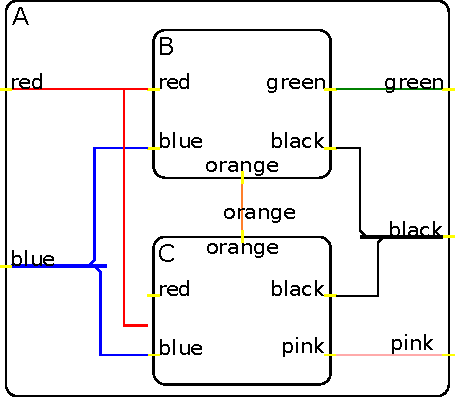
\includegraphics[width=0.5\linewidth]{hierColor.pdf}
\caption{TODO.
\label{fig:hierColor}}
\end{figure} % }}}

% }}} sec:workedExample

\subsubsection{Tool Support} % {{{
\label{sec:HungarianNotation_toolSupport}
The only class of tools which care about naming conventions are those which
perform stylistic lint checks.

% TODO: Tidy up description style.
\begin{description}
%\item[Icarus, AKA iverilog (\gls{FOSS})]
%  Simulator.
%  Specific flag (\texttt{-E}) allows enables use as a standalone pre-processor.
\item[Verilator (\gls{FOSS})]
  Fast, 2-state simulator.
  The \texttt{{-}{-}lint-only} flag invokes only structural lint checks such as
  unconnected module ports and mismatching widths.
  No stylistic checks are performed.
\item[svlint]
  Linter.
  \TODO{Naming convention checks are WIP.}
%\item[Yosys - (\gls{FOSS})]
%  Generic synthesis tool primarily targeting Lattice and Xilinx \glspl{FPGA}.
\item[HAL 20.03 (Cadence)]
  Linter.
%\item[JasperGold 2020.03 (Cadence)]
%  Formal proof assistant.
%\item[Xcelium 20.03 (Cadence)]
%  Simulator.
%\item[Formalpro v2020.1 (Siemens)]
%  Equivalence checker.
%\item[Design Compiler TODO (Synopsys)]
%  Generic synthesis tool for \glspl{ASIC}.
%  \TODO{Full support for \gls{DFF} macros.???}
\item[Spyglass 2020.12 (Synopsys)]
  Linter.
%\item[VCS 2018.09 (Synopsys)]
%  Simulator.
%\item[Vivado 2018.02 (Xilinx)]
%  Complete \gls{FPGA} flow including synthesis (Synplify Pro) and simulation.
\end{description}

% }}} sec:toolSupport

\subsubsection{Potential Problems} % {{{
\label{sec:HungarianNotation_potentialProblems}
\TODO{Potential Problems}

% }}} sec:potentialProblems

% }}} sec:discussion

\subsection{Conclusion} % {{{
\label{sec:HungarianNotation_conclusion}
\TODO{Conclusion}

% }}} sec:conclusion

% }}} sec:HungarianNotation

\section{Simple, Always} % {{{
\label{sec:SimpleAlways}
\TODO{Introduction}

\paragraph{Problem Description} % {{{
\label{sec:SimpleAlways_problem}
\TODO{Problem Description}

% }}} sec:SimpleAlways_problem

\paragraph{Objective} % {{{
\label{sec:SimpleAlways_objective}
\TODO{Objective}

% }}} sec:SimpleAlways_objective

\paragraph{Approach} % {{{
\label{sec:SimpleAlways_approach}
\TODO{Approach}
\TODO{Restriction on structure of always blocks.}
\TODO{Restriction on use of wire/reg/logic/var.}

% }}} sec:aSimpleAlways_pproach

\subsection{Background and Related Work} % {{{
\label{sec:SimpleAlways_background}
\TODO{Background}
\TODO{assign, always, always\_comb, ...}
\TODO{var vs net}

% }}} sec:SimpleAlways_background

\subsection{Methodology} % {{{
\label{sec:SimpleAlways_methodology}
\TODO{Methodology}

% }}} sec:SimpleAlways_methodology

\subsection{Discussion} % {{{
\label{sec:SimpleAlways_discussion}
\TODO{Discussion}

\subsubsection{Worked Examples} % {{{
\label{sec:SimpleAlways_workedExamples}
\TODO{Worked Examples}

% }}} sec:SimpleAlways_workedExample

\subsubsection{Tool Support} % {{{
\label{sec:SimpleAlways_toolSupport}
The only class of tools which care about naming conventions are those which
perform stylistic lint checks.

% TODO: Tidy up description style.
\begin{description}
%\item[Icarus, AKA iverilog (\gls{FOSS})]
%  Simulator.
%  Specific flag (\texttt{-E}) allows enables use as a standalone pre-processor.
\item[Verilator (\gls{FOSS})]
  Fast, 2-state simulator.
\item[svlint]
  Linter.
  \TODO{Naming convention checks are WIP.}
%\item[Yosys - (\gls{FOSS})]
%  Generic synthesis tool primarily targeting Lattice and Xilinx \glspl{FPGA}.
\item[HAL 20.03 (Cadence)]
  Linter.
%\item[JasperGold 2020.03 (Cadence)]
%  Formal proof assistant.
%\item[Xcelium 20.03 (Cadence)]
%  Simulator.
%\item[Formalpro v2020.1 (Siemens)]
%  Equivalence checker.
%\item[Design Compiler TODO (Synopsys)]
%  Generic synthesis tool for \glspl{ASIC}.
%  \TODO{Full support for \gls{DFF} macros.???}
\item[Spyglass 2020.12 (Synopsys)]
  Linter.
%\item[VCS 2018.09 (Synopsys)]
%  Simulator.
%\item[Vivado 2018.02 (Xilinx)]
%  Complete \gls{FPGA} flow including synthesis (Synplify Pro) and simulation.
\end{description}

% }}} sec:SimpleAlways_toolSupport

\subsubsection{Potential Problems} % {{{
\label{sec:SimpleAlways_potentialProblems}
\TODO{Potential Problems}

% }}} sec:SimpleAlways_potentialProblems

% }}} sec:SimpleAlways_discussion

\subsection{Conclusion} % {{{
\label{sec:SimpleAlways_conclusion}
\TODO{Conclusion}

% }}} sec:SimpleAlways_conclusion

% }}} sec:SimpleAlways

\section{Boring Flops} % {{{
\label{sec:BoringFlops}
\TODO{Introduction}

\paragraph{Problem Description} % {{{
\label{sec:BoringFlops_problem}
\TODO{Problem Description}

% }}} sec:BoringFlops_problem

\paragraph{Objective} % {{{
\label{sec:BoringFlops_objective}
\TODO{Objective}

% }}} sec:BoringFlops_objective

\paragraph{Approach} % {{{
\label{sec:BoringFlops_approach}
\TODO{Approach}

% }}} sec:BoringFlops_approach

\subsection{Background and Related Work} % {{{
\label{sec:BoringFlops_background}
\TODO{Background}

% }}} sec:BoringFlops_background

\subsection{Methodology} % {{{
\label{sec:BoringFlops_methodology}
\TODO{Methodology}

% }}} sec:BoringFlops_methodology

\subsection{Discussion} % {{{
\label{sec:BoringFlops_discussion}
\TODO{Discussion}

\subsubsection{Worked Examples} % {{{
\label{sec:BoringFlops_workedExamples}
\TODO{Worked Examples}

% }}} sec:BoringFlops_workedExample

\subsubsection{Tool Support} % {{{
\label{sec:BoringFlops_toolSupport}
These selected \gls{FOSS} and commercial tools have been specifically tested,
and examples of their usage is contained in \texttt{dmpvl/mk/lint.mk}.
Full support is provided by all modern tools when the appropriate flags are
used for System Verilog mode.
Only the oldest tested version of each tool is shown because no regressions
have been seen in newer versions.

% TODO: Tidy up description style.
\begin{description}
\item[Icarus, AKA iverilog (\gls{FOSS})]
  Simulator.
  Specific flag (\texttt{-E}) allows enables use as a standalone pre-processor.
\item[Verilator (\gls{FOSS})]
  Fast, 2-state simulator.
  Specific flag (\texttt{-E}) allows enables use as a standalone pre-processor.
\item[svlint]
  Linter.
  \TODO{Naming convention checks are WIP.}
\item[Yosys - (\gls{FOSS})]
  Generic synthesis tool primarily targeting Lattice and Xilinx \glspl{FPGA}.
\item[HAL 20.03 (Cadence)]
  Linter.
\item[JasperGold 2020.03 (Cadence)]
  Formal proof assistant.
\item[Xcelium 20.03 (Cadence)]
  Simulator.
\item[Formalpro v2020.1 (Siemens)]
  Equivalence checker.
\item[Design Compiler TODO (Synopsys)]
  Generic synthesis tool for \glspl{ASIC}.
  \TODO{Full support for \gls{DFF} macros.???}
\item[Spyglass 2020.12 (Synopsys)]
  Linter.
\item[VCS 2018.09 (Synopsys)]
  Simulator.
\item[Vivado 2018.02 (Xilinx)]
  Complete \gls{FPGA} flow including synthesis (Synplify Pro) and simulation.
\end{description}

% }}} sec:BoringFlops_toolSupport

\subsubsection{Potential Problems} % {{{
\label{sec:BoringFlops_potentialProblems}
\TODO{Potential Problems}

% }}} sec:BoringFlops_potentialProblems

% }}} sec:BoringFlops_discussion

\subsection{Conclusion} % {{{
\label{sec:BoringFlops_conclusion}
\TODO{Conclusion}

% }}} sec:BoringFlops_conclusion

% }}} sec:BoringFlops

\section{Synthesisable Properties} % {{{
\label{sec:SynthesisableProperties}
\TODO{Introduction}

\paragraph{Problem Description} % {{{
\label{sec:SynthesisableProperties_problem}
\TODO{Problem Description}

% }}} sec:SynthesisableProperties_problem

\paragraph{Objective} % {{{
\label{sec:SynthesisableProperties_objective}
\TODO{Objective}

% }}} sec:SynthesisableProperties_objective

\paragraph{Approach} % {{{
\label{sec:SynthesisableProperties_approach}
\TODO{Approach}

% }}} sec:SynthesisableProperties_approach

\subsection{Background and Related Work} % {{{
\label{sec:SynthesisableProperties_background}
\TODO{Background}

% }}} sec:SynthesisableProperties_background

\subsection{Methodology} % {{{
\label{sec:SynthesisableProperties_methodology}
\TODO{Methodology}

% }}} sec:SynthesisableProperties_methodology

\subsection{Discussion} % {{{
\label{sec:SynthesisableProperties_discussion}
\TODO{Discussion}

\subsubsection{Worked Examples} % {{{
\label{sec:SynthesisableProperties_workedExamples}
\TODO{Worked Examples}

% }}} sec:SynthesisableProperties_workedExample

\subsubsection{Tool Support} % {{{
\label{sec:SynthesisableProperties_toolSupport}
\TODO{Simulators with any assert support are good.}
\TODO{Formal property checking, synth, PnR false path}
\TODO{Simulators with any assert support are good.}

% TODO: Tidy up description style.
\begin{description}
%\item[Icarus, AKA iverilog (\gls{FOSS})]
%  Simulator.
%  Specific flag (\texttt{-E}) allows enables use as a standalone pre-processor.
\item[Verilator (\gls{FOSS})]
  Fast, 2-state simulator.
%\item[svlint]
%  Linter.
%  \TODO{Naming convention checks are WIP.}
%\item[Yosys - (\gls{FOSS})]
%  Generic synthesis tool primarily targeting Lattice and Xilinx \glspl{FPGA}.
%\item[HAL 20.03 (Cadence)]
%  Linter.
%\item[JasperGold 2020.03 (Cadence)]
%  Formal proof assistant.
%\item[Xcelium 20.03 (Cadence)]
%  Simulator.
%\item[Formalpro v2020.1 (Siemens)]
%  Equivalence checker.
%\item[Design Compiler TODO (Synopsys)]
%  Generic synthesis tool for \glspl{ASIC}.
%  \TODO{Full support for \gls{DFF} macros.???}
%\item[Spyglass 2020.12 (Synopsys)]
%  Linter.
%\item[VCS 2018.09 (Synopsys)]
%  Simulator.
%\item[Vivado 2018.02 (Xilinx)]
%  Complete \gls{FPGA} flow including synthesis (Synplify Pro) and simulation.
\end{description}

% }}} sec:SynthesisableProperties_toolSupport

\subsubsection{Potential Problems} % {{{
\label{sec:SynthesisableProperties_potentialProblems}
\TODO{Potential Problems}

% }}} sec:SynthesisableProperties_potentialProblems

% }}} sec:SynthesisableProperties_discussion

\subsection{Conclusion} % {{{
\label{sec:SynthesisableProperties_conclusion}
\TODO{Conclusion}

% }}} sec:SynthesisableProperties_conclusion

% }}} sec:SynthesisableProperties


% {{{ epilog

\ifdefined\ShowReferences
  \newpage
  \bibliographystyle{shr/tex/IEEEtran}
  \bibliography{shr/refs}{} % refs.bib
\fi

\ifdefined\ShowGlossary
  \clearpage
  \phantomsection
  \addcontentsline{toc}{section}{Glossary}
  \printnoidxglossary[sort=letter]
\fi

% }}} epilog

\end{document}
